

%%%%%%%% Chapters %%%%%%%%%%%%
%% Results
\chapter{Results}
\label{chap:results}

Now that we have defined the encoding similarity between two sentences, we are able to systematically compare encoded sentences in the Europarl and Seed datasets to test the hypothesis that sentences of the same meaning are similarly encoded. But just because the encoding similarity calculation produces values in the range [-1.0, 1.0], it is not necessarily the case that a positive encoding similarity indicates that two encodings are more similar than dissimilar in the context of a particular model. It may be that the encoder has learned to produce token encoding vectors with only non-negative elements, in which case the minimum possible similarity becomes 0.0. That is to say that calculation of encoding similarity between sentences of the same meaning in different languages will not itself support or contradict the hypothesis. 

In order to show how encoding similarity and meaning are related, it is necessary to compare the encoding similarity among sentences grouped by some other feature to the similarity among sentences of the same meaning. We will calculate the similarity between pairs of sentences with three types of relationships:

\begin{enumerate}
  \item Sentences with the same meaning in different languages (interlingual)
  \item Sentences with different meanings in the same language (intralingual)
  \item Sentences with different meanings in different languages (spurious)
\end{enumerate}

The missing fourth group, sentences with the same meaning in the same language, is trivial. The encoding similarity between a sentence and itself is 1.0, regardless of its meaning or language. It might be interesting to study the encodings of sentences with the same semantic meaning but written slightly differently, but our parallel corpora contain only one version of each sentence per language.

\section{Random Variables}
By calculating the encoding similarity in the groups listed above, we define three random variables, X, Y, and Z. Random variable X represents interlingual encoding similarity, Y represents intralingual encoding similarity, and Z represents spurious encoding similarity. The expected value of each random variable is the average encoding similarity over a large set of sentences. Thus we produce several statistics, comparable by dataset, model size, language, language pair, or other data characteristics. 

\subsection{Random Variable X: Interlingual Similarity}

Interlingual similarity can be viewed at three levels: 

\begin{itemize}
	\item A particular language’s average similarity to one other language. 
	\item A particular language’s average similarity to all other languages.
	\item The average similarity between each pair of languages.
\end{itemize}

The starting point for these three types of statistics is bullet point 1 - pairwise encoding similarity. We calculate pairwise similarity simply by taking the arithmetic mean of the similarities between each pair of parallel sentences. In a dataset with N languages, there are (N * (N-1))/2 language pairs. We can display the pairwise similarities on a square heatmap, which, because pairwise similarity is symmetrical, will exhibit symmetry along the diagonal. The squares along the diagonal have the maximum similarity of 1.0 because they represent the previously-mentioned trivial self-similarity of the sentences in each language.  

The second kind of interlingual similarity, a particular language’s average similarity to all other languages, is easily calculated by taking the arithmetic mean of each row. In this example, Estonian has the lowest average interlingual similarity, 0.590, and English has the highest, 0.763. (maybe ok to keep values)

By taking yet another average, we can distill all this information into a single statistic, the average encoding similarity between all pairs of sentences with the same meaning; for this set of 10,000 Europarl sentences encoded by the 600-million-parameter NLLB model, that value is 0.699. (maybe exclude last sentence)

\subsection{Random Variable Y: Intralingual Similarity}

use pseudocode algorithm for rejection sampling thing

Although calculation of intralingual similarity does not require comparison of sentences with the same meaning, other variables should be kept constant. A feature of sentences with the same meaning is that they tend to have similar lengths. thus, we choose pairs not by matching sentences to arbitrary sentences from the same language, but by sampling by length according to the distributions we measure in their dataset. For each dataset, Seed and Europarl, we sampled pairs of sentences for comparison not only with the criterion that they have officially different meanings, but that they also have a minimum edit distance between them. The second stipulation is more likely to matter in the Europarl dataset, in which many diplomatic phrases are repeated, possibly with very small variations. After producing a number of pairs equivalent to the number of sentences per language in the original dataset, intralingual similarity is calculated as the average of the encoding similarities of each pair.  

Intralingual similarity is calculated by language, not by language pair. Thus we can compare the intralingual similarity of each language to its average interlingual similarity and the overall average intralingual similarity to the overall average interlingual similarity. 

\subsection{Random Variable Z: Spurious Similarity}

Spurious similarity involves calculations between pairs of languages (like interlingual similarity) and length-based sampling to select sets of sentences with different meanings (like intralingual similarity). We sample N sentences per language, again with the stipulations that they neither have identical meaning nor very similar text. Then we produce the same three types of statistics as we do with random variable X: language pair similarity, average language pair similarity by language, and an overall average similarity. That is, we produce another heatmap of similarities, an average for each language, and finally a single statistic for the dataset. 

\section{Null Hypotheses}

With the three random variables X, Y, and Z, we define three kinds of statistics about a dataset. Our hypothesis, that multilingual encoders encode sentences with the same meaning similarly, only refers only the first random variable, interlingual similarity, but it also involves the other two. We must show that interlingual, intralingual, and spurious similarities are not equal, that is, we aim to reject the following null hypotheses which would contradict our hypothesis:

	\begin{enumerate}
		\item The expected values of X and Y are equal.
		\item The expected values of X and Z are equal.
		\item The expected values of Y and Z are equal.
	\end{enumerate}
	
Regarding null hypotheses one and two, we'd actually like to show that the expected value of X is higher than that of Y or Z in order to accept our hypothesis. Null hypothesis three is not strictly necessary, but we have all the data necessary to  less bearing on our hypothesis, but investigating it may help to provide a clearer picture of how multilingual encoders train.

\subsection{Null Hypothesis 1}
We would like to show that the expected value of random variables X and Y are not equal, i.e. that average interlingual similarity is not equal to average intralingual similarity. Since intralingual singularity experiments do not produce statistics by language pair, the first type of statistic produced for interlingual similarity (which does represent language pair encoding similarity) will not be directly useful. Rather, we will use the average similarity by language as well as dataset averages to compare interlingual and intralingual encoding similarities. 

A graphical comparison of per language averages clearly shows a difference between interlingual and intralingual similarities.

\begin{figure}[htbp]
    \centering
    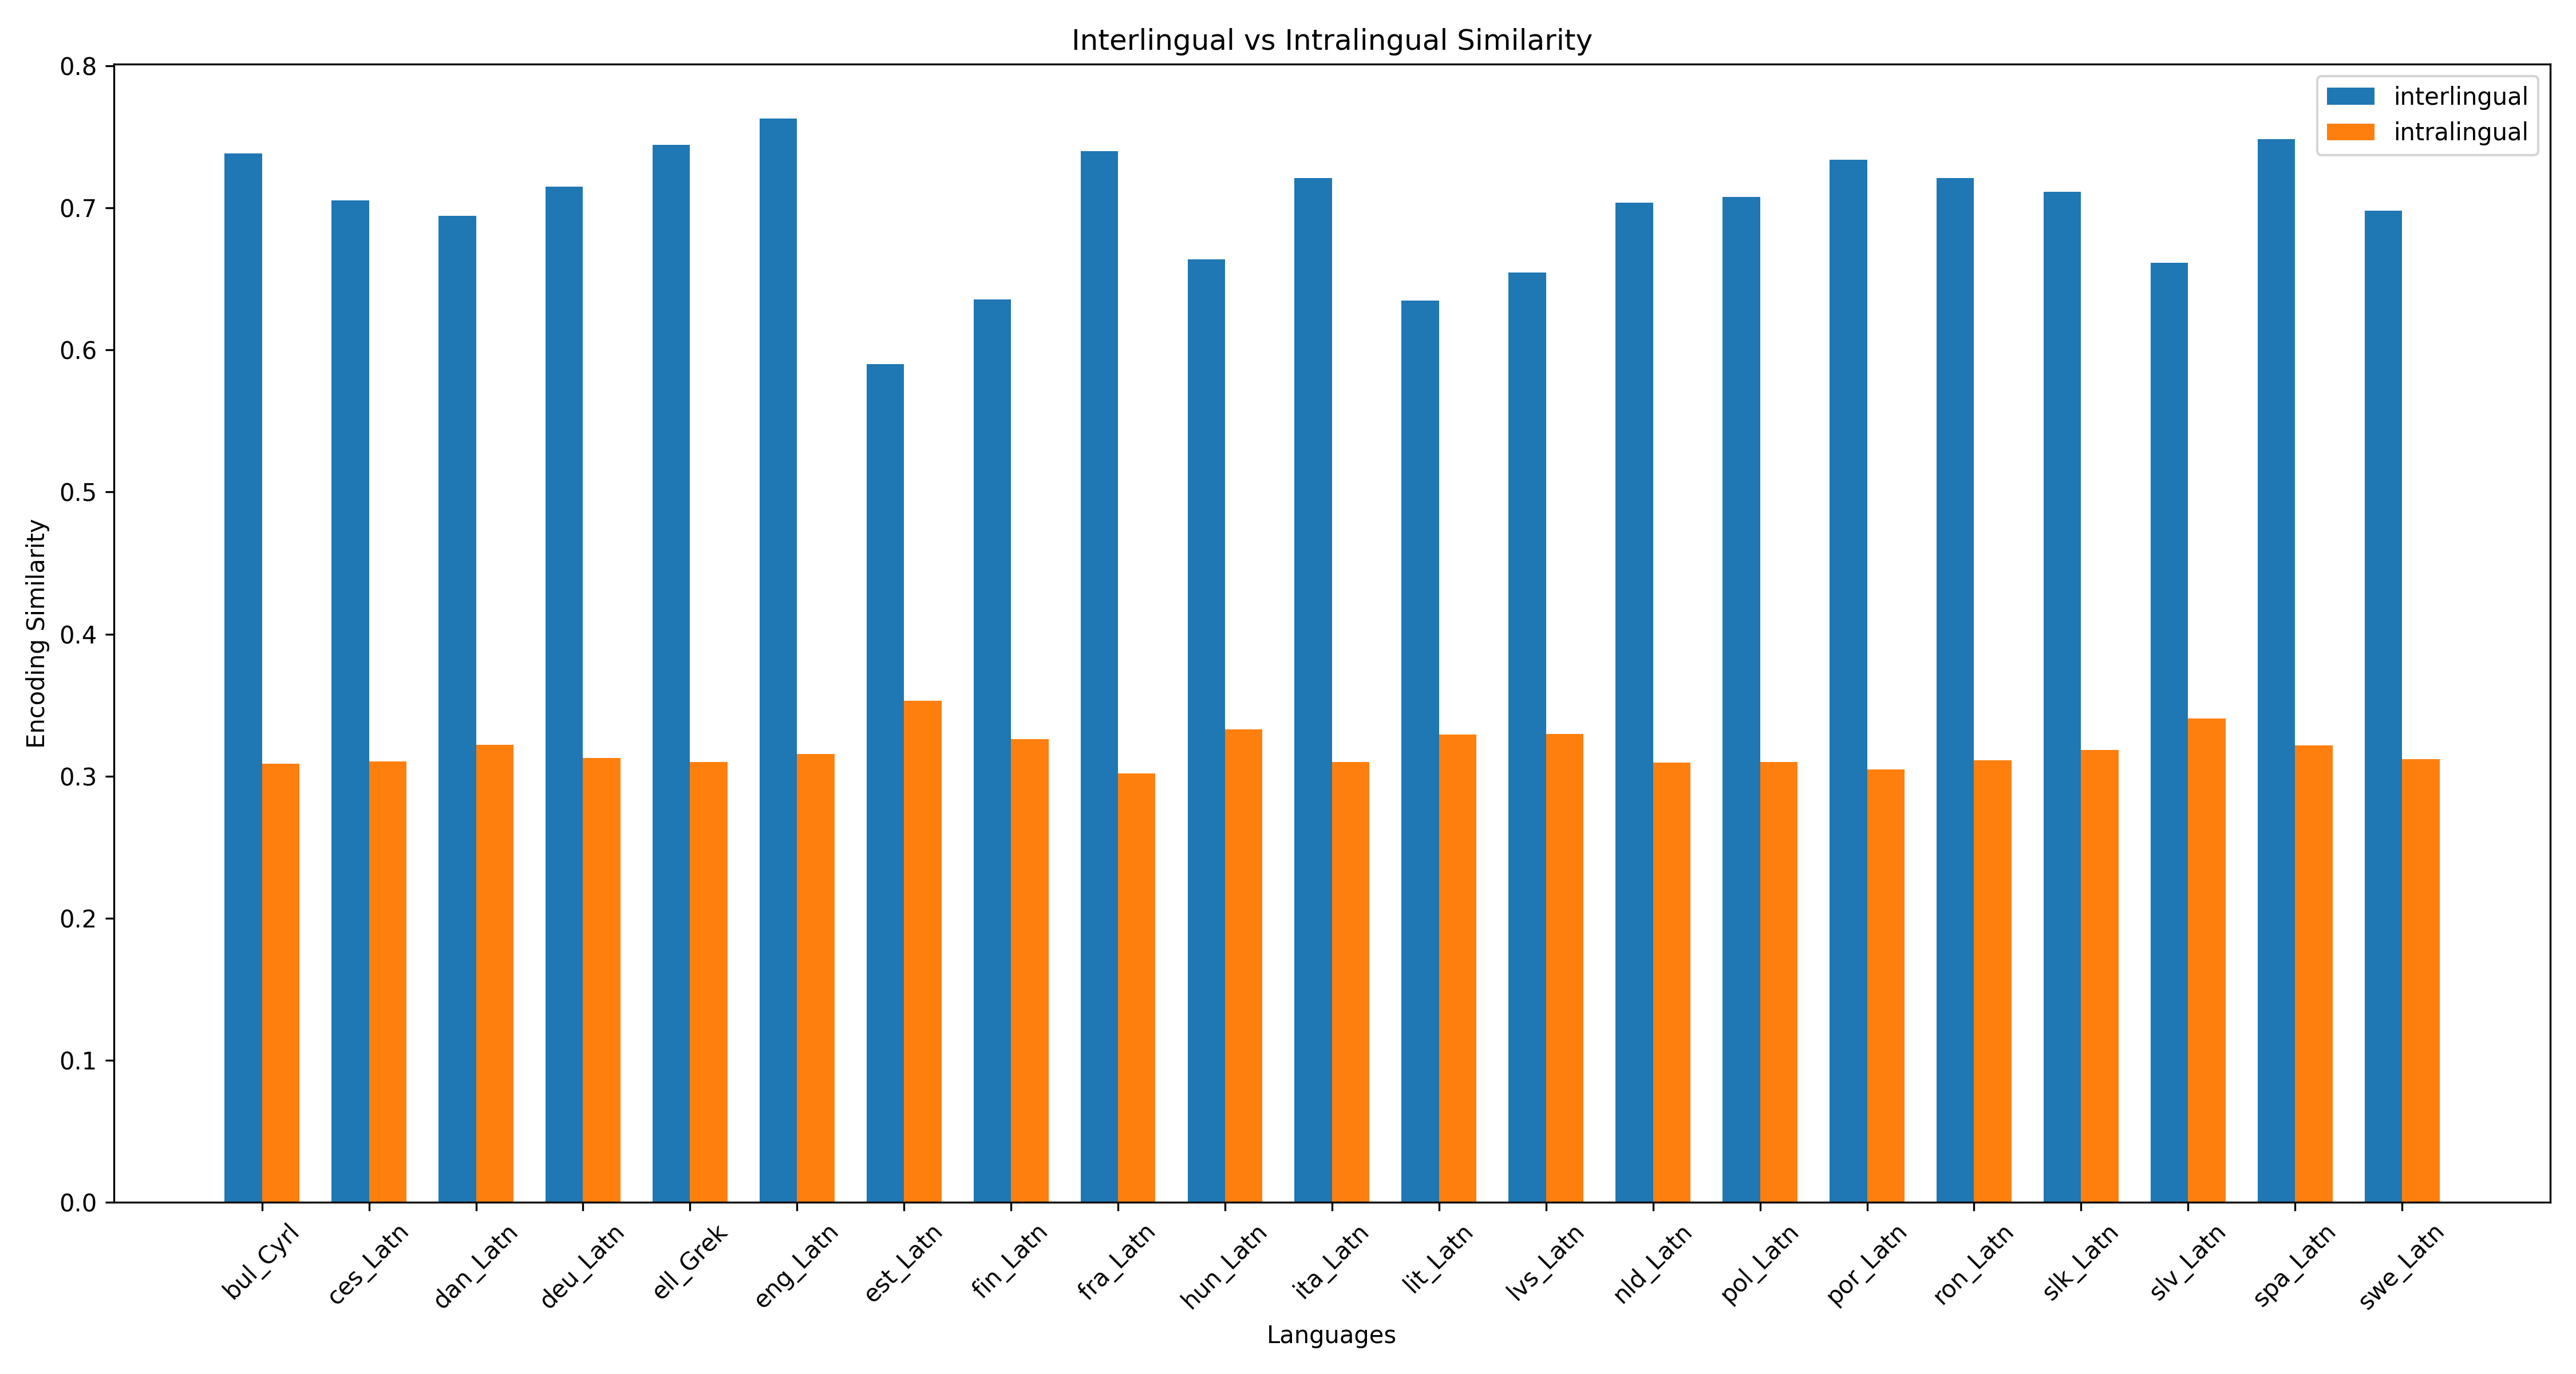
\includegraphics[width=\textwidth]{images/europarl_rv1.png}
    \caption{Interlingual vs intralingual similarity by language in the Europarl dataset}
    \label{fig:europarl_rv1}
\end{figure}



\begin{figure}[htbp]
    \centering
    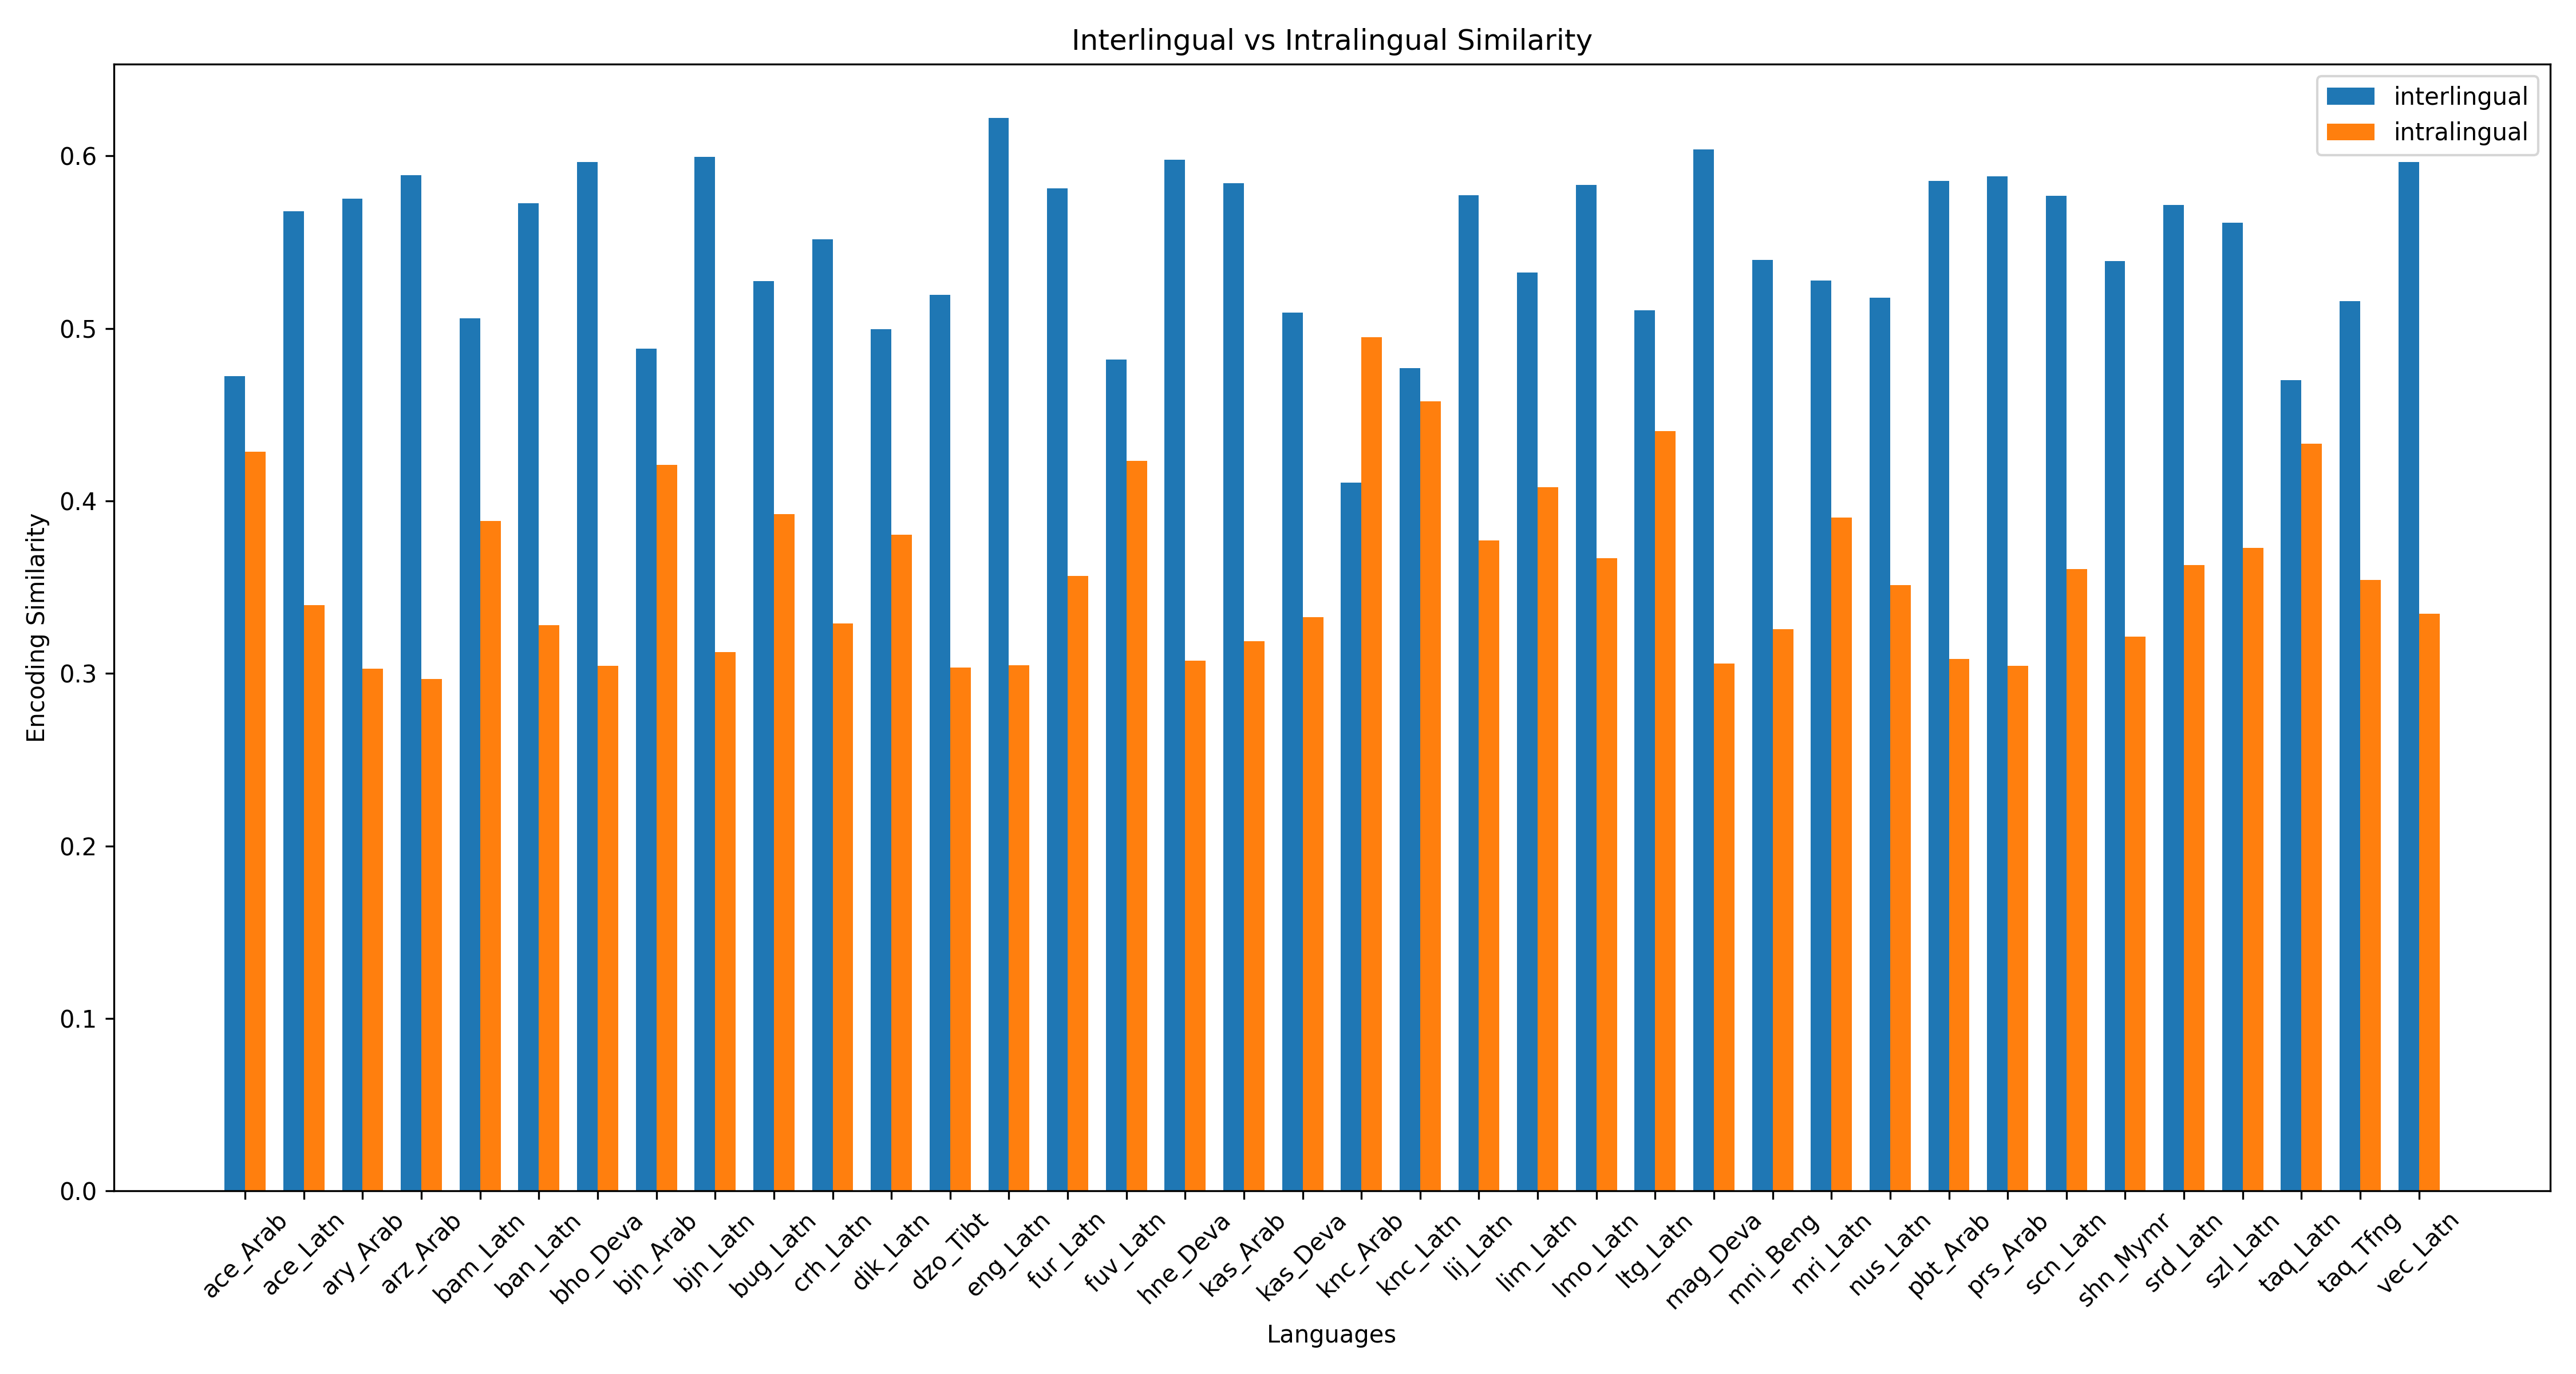
\includegraphics[width=\textwidth]{images/seed_rv1.png}
    
    \caption{Interlingual vs intralingual similarity by language in the Seed dataset}
    \label{fig:seed_rv1}
\end{figure}


In the Europarl dataset, the average interlingual mean across languages, that is, the mean encoding similarity between encodings of sentences with the same meaning in different languages, is 0.699, while the mean intralingual similarity is 0.319. [insert stats here just to say that the result is significant based on a t-test]. For the Seed dataset, the mean interlingual encoding similarity is 0.545 while the mean intralingual encoding similarity is 0.359. [same stats work]. According to these t-tests, we reject the null hypothesis that the expected values of interlingual and intralingual similarity are equal.

It is worth noting that the gap between these two values is significantly smaller in the Seed dataset than in the Europarl dataset. One of the Seed languages, knc\_Arab, even has higher intralingual similarity than interlingual similarity, which is not the case for any of the Europarl languages. These differences can most likely be explained by the fact that the Seed languages are all low-resource and that the Europarl languages are all high-resource (in the context of NLLB). Sentences from languages which are better understood by the NLLB models are better grouped by meaning than by language, and this phenomenon falls on a spectrum. The outlier in the Seed dataset, knc\_Arab (which stands for Central Kanuri in Arabic script) has among the worst performance in xx-English and English-xx translation tasks. On the other end of the spectrum, we could place Spanish, whose average interlingual similarity is more than double its intralingual similarity.


\subsection{Null Hypothesis 2}
In addition to showing that the expected values for average interlingual and average intralingual similarities are not equal, we would like to show that the expected values for interlingual and spurious similarity are not equal. Thus we must compare the average similarity of sentences with the same meaning in different languages to the average similarity of sentences with neither a common language nor meaning. As outlined above, these unrelated sentences were selected using rejection sampling, which takes into account sentence length (based on measured characteristics of the Europarl and Seed datasets) and edit distance, ensuring that paired sentences are both similar in length and lexically distant. 

We calculate that the average interlingual similarity in the Europarl dataset is 0.699 and that the average spurious similarity is 0.359. In the Seed dataset, the average interlingual similarity is 0.545 and the average spurious similarity is 0.348. Using the method of t-testing described above, we find this these differences statistically significant with p-values FILLINBLANK and FILLINBLANK. Thus null hypothesis 2, that the random variables representing average interlingual and spurious similarity have the same expected values, can be rejected. 

A heatmap makes an effective visual reference for interlingual and spurious similarity calculations by language pair. According to our hypothesis, we should see an overall brighter heatmaps representing interlingual similarity than ones representing spurious similarity. Of course, we can compare overall averages for each dataset, but more specific qualities of the data are legible in this two-dimensional format. The following clustered heatmaps display the interlingual and spurious similarities of language pair in both of our two datasets. 

\begin{figure}[htbp]
    \centering
    \includegraphics[width=0.7\textwidth]{images/rv2_europarl_inter.png}
    \caption{Interlingual similarity by language pair in the Europarl dataset}
    \label{fig:europarl_rv2_inter}
\end{figure}

\begin{figure}[htbp]
    \centering
    \includegraphics[width=0.7\textwidth]{images/rv2_europarl_spurious.png}
    
    \caption{Spurious similarity by language pair in the Europarl dataset}
    \label{fig:europarl_rv2_spurious}
\end{figure}



\begin{figure}[htbp]
    \centering
    \includegraphics[width=0.7\textwidth]{images/rv2_seed_inter.png}
    \caption{Interlingual similarity by language pair in the Seed dataset}
    \label{fig:europarl_rv2_inter}
\end{figure}

\begin{figure}[htbp]
    \centering
    \includegraphics[width=0.7\textwidth]{images/rv2_seed_spurious.png}
    
    \caption{Spurious similarity by language pair in the Seed dataset}
    \label{fig:europarl_rv2_spurious}
\end{figure}

The interlingual heatmaps clearly show brighter, i.e. higher, values than the spurious ones, but they also display patterns in the data. There is greater differentiation by language in the interlingual heatmap. This is a good indication that spurious similarity has the behavior we expect -- sentences with neither a common language nor meaning follow no pattern clearly governed by language. We can observe some noise, but that is entirely to be expected. Corresponding graphs for the 1.3 billion parameter NLLB model can be found in the appendix.

\subsection{Null Hypothesis 3}

Null hypothesis 3 states that the expected values of random variables Y (intralingual similarity) and Z (spurious similarity) are equal. The meaning of this statement and of its rejection are less crucial to our main hypothesis than null hypotheses 1 and 2, but since we have the data and expect these values to differ, it is worth comparing these two random variables. Is intralingual similarity higher on average or lower than spurious similarity? The answer to this question might indicate what effect grouping sentences in space based on their language has on the course of training.

\begin{figure}[htbp]
    \centering
    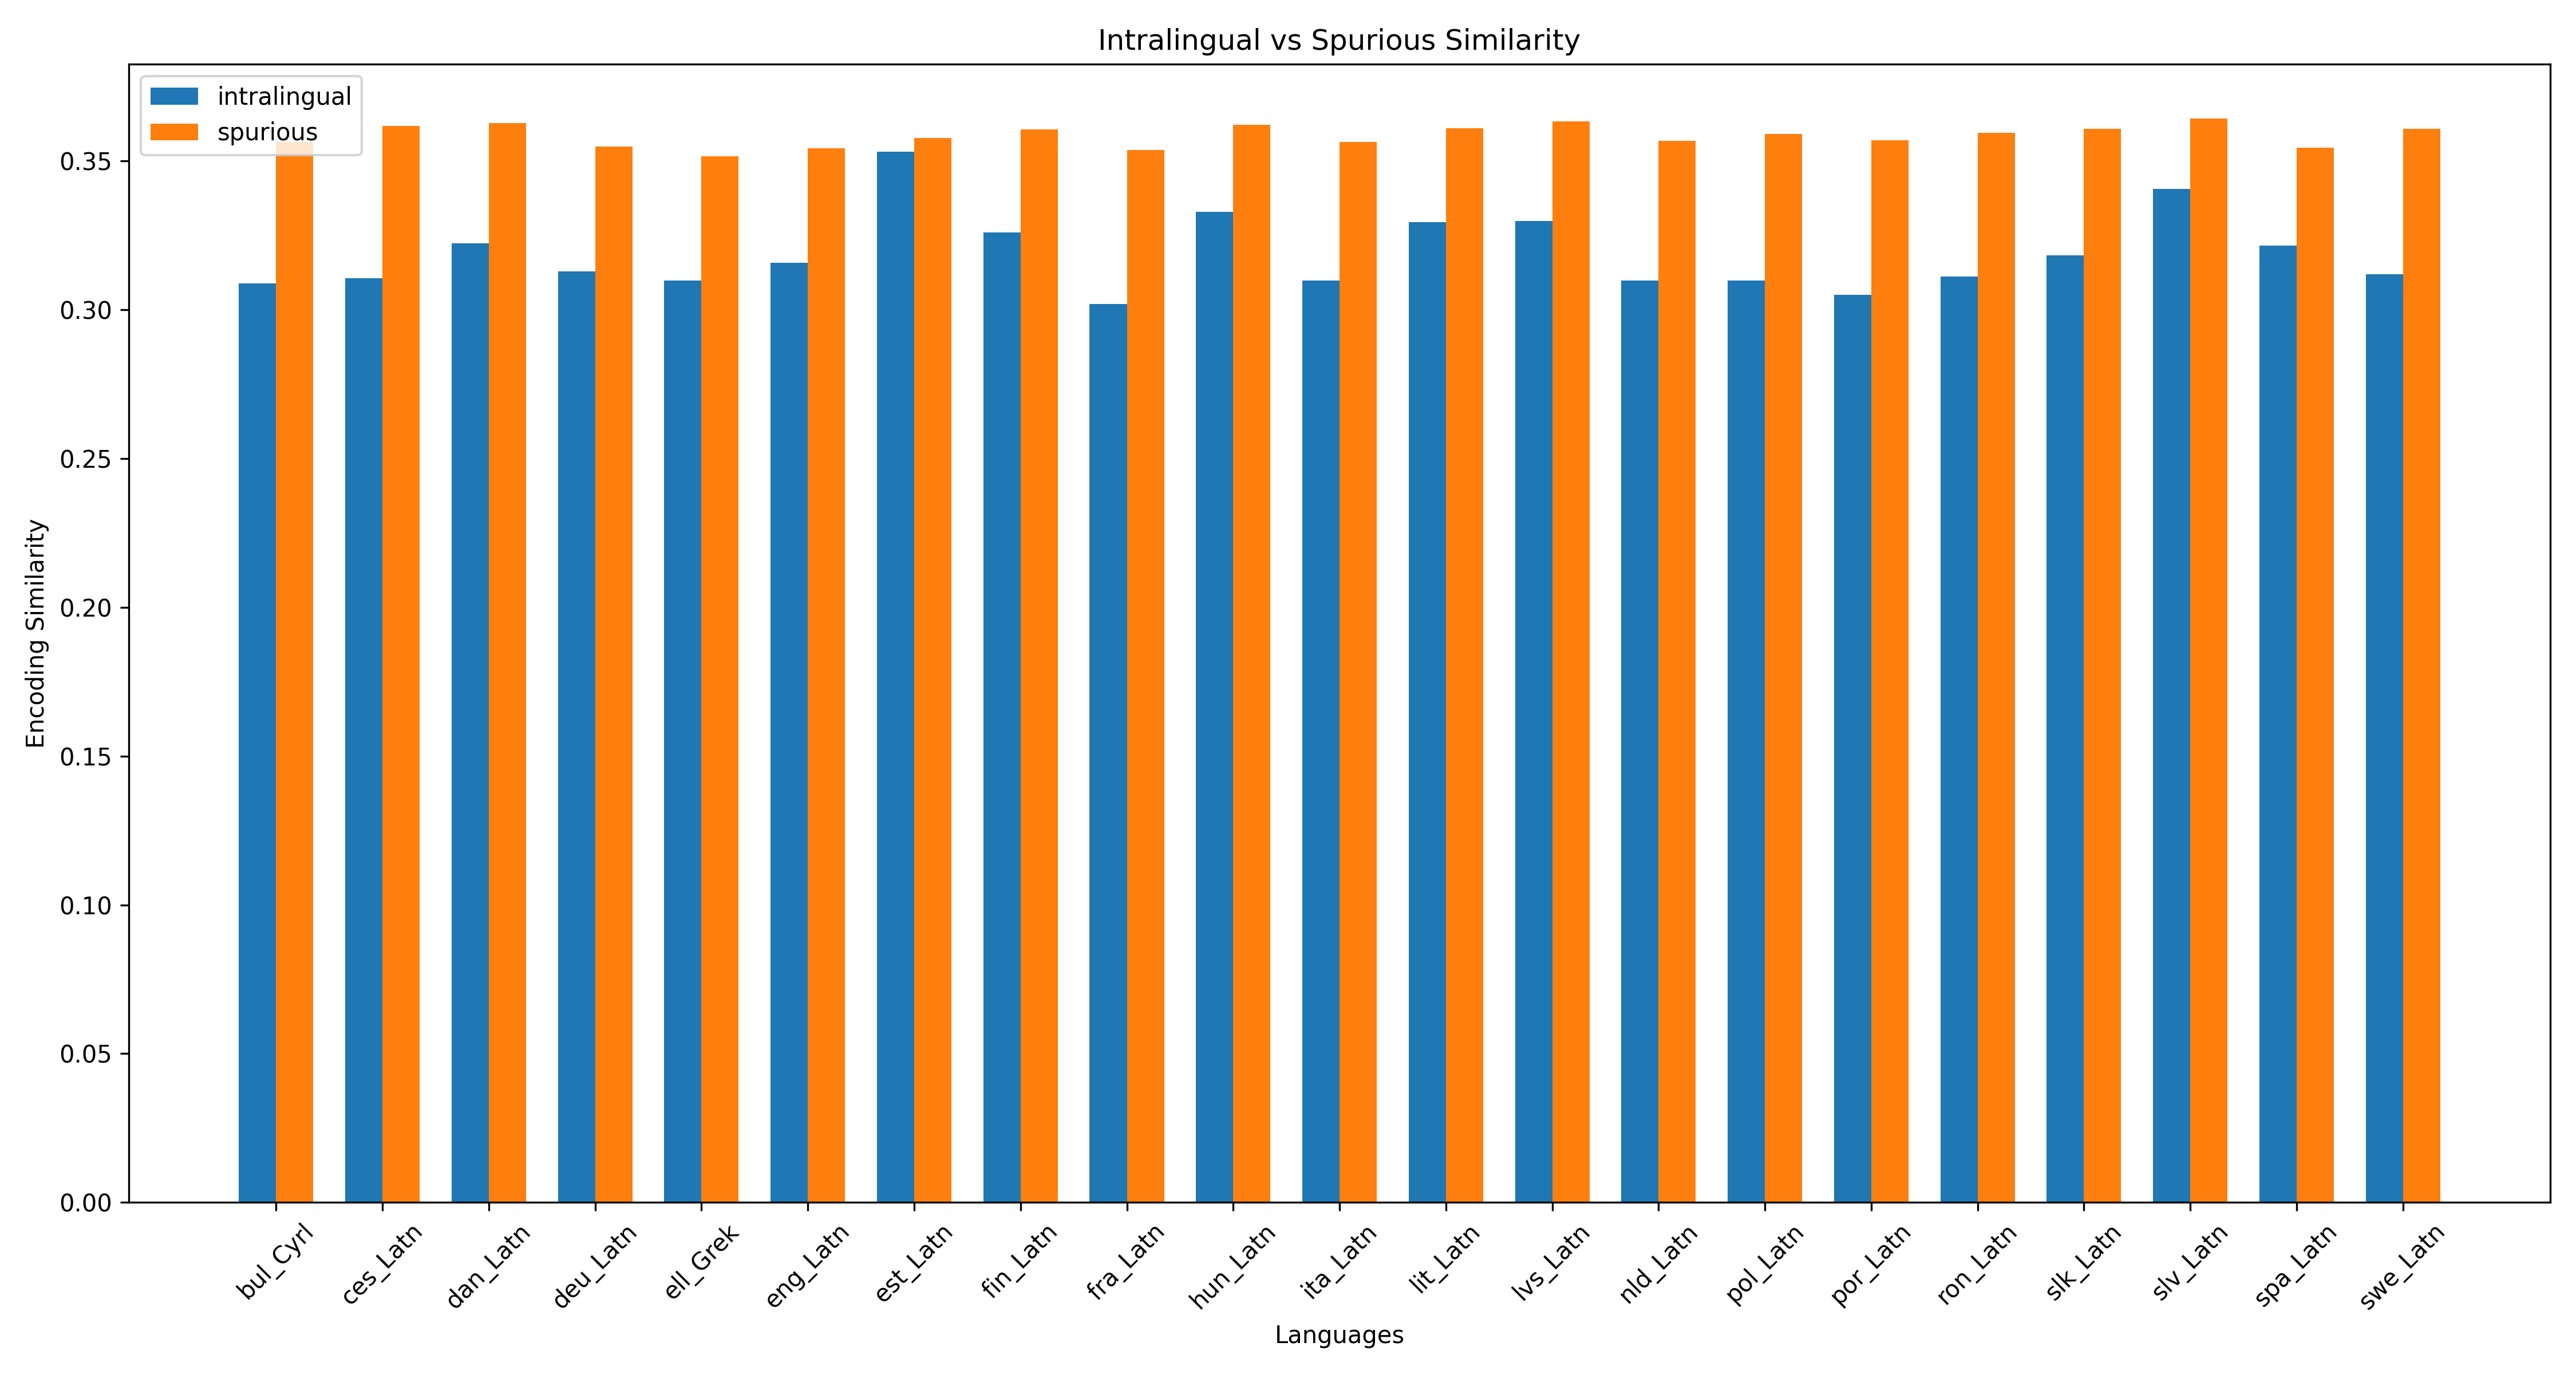
\includegraphics[width=\textwidth]{images/rv3_europarl.png}
    \caption{Intralingual vs spurious similarity by language in the Europarl dataset}
    \label{fig:europarl_rv3}
\end{figure}



\begin{figure}[htbp]
    \centering
    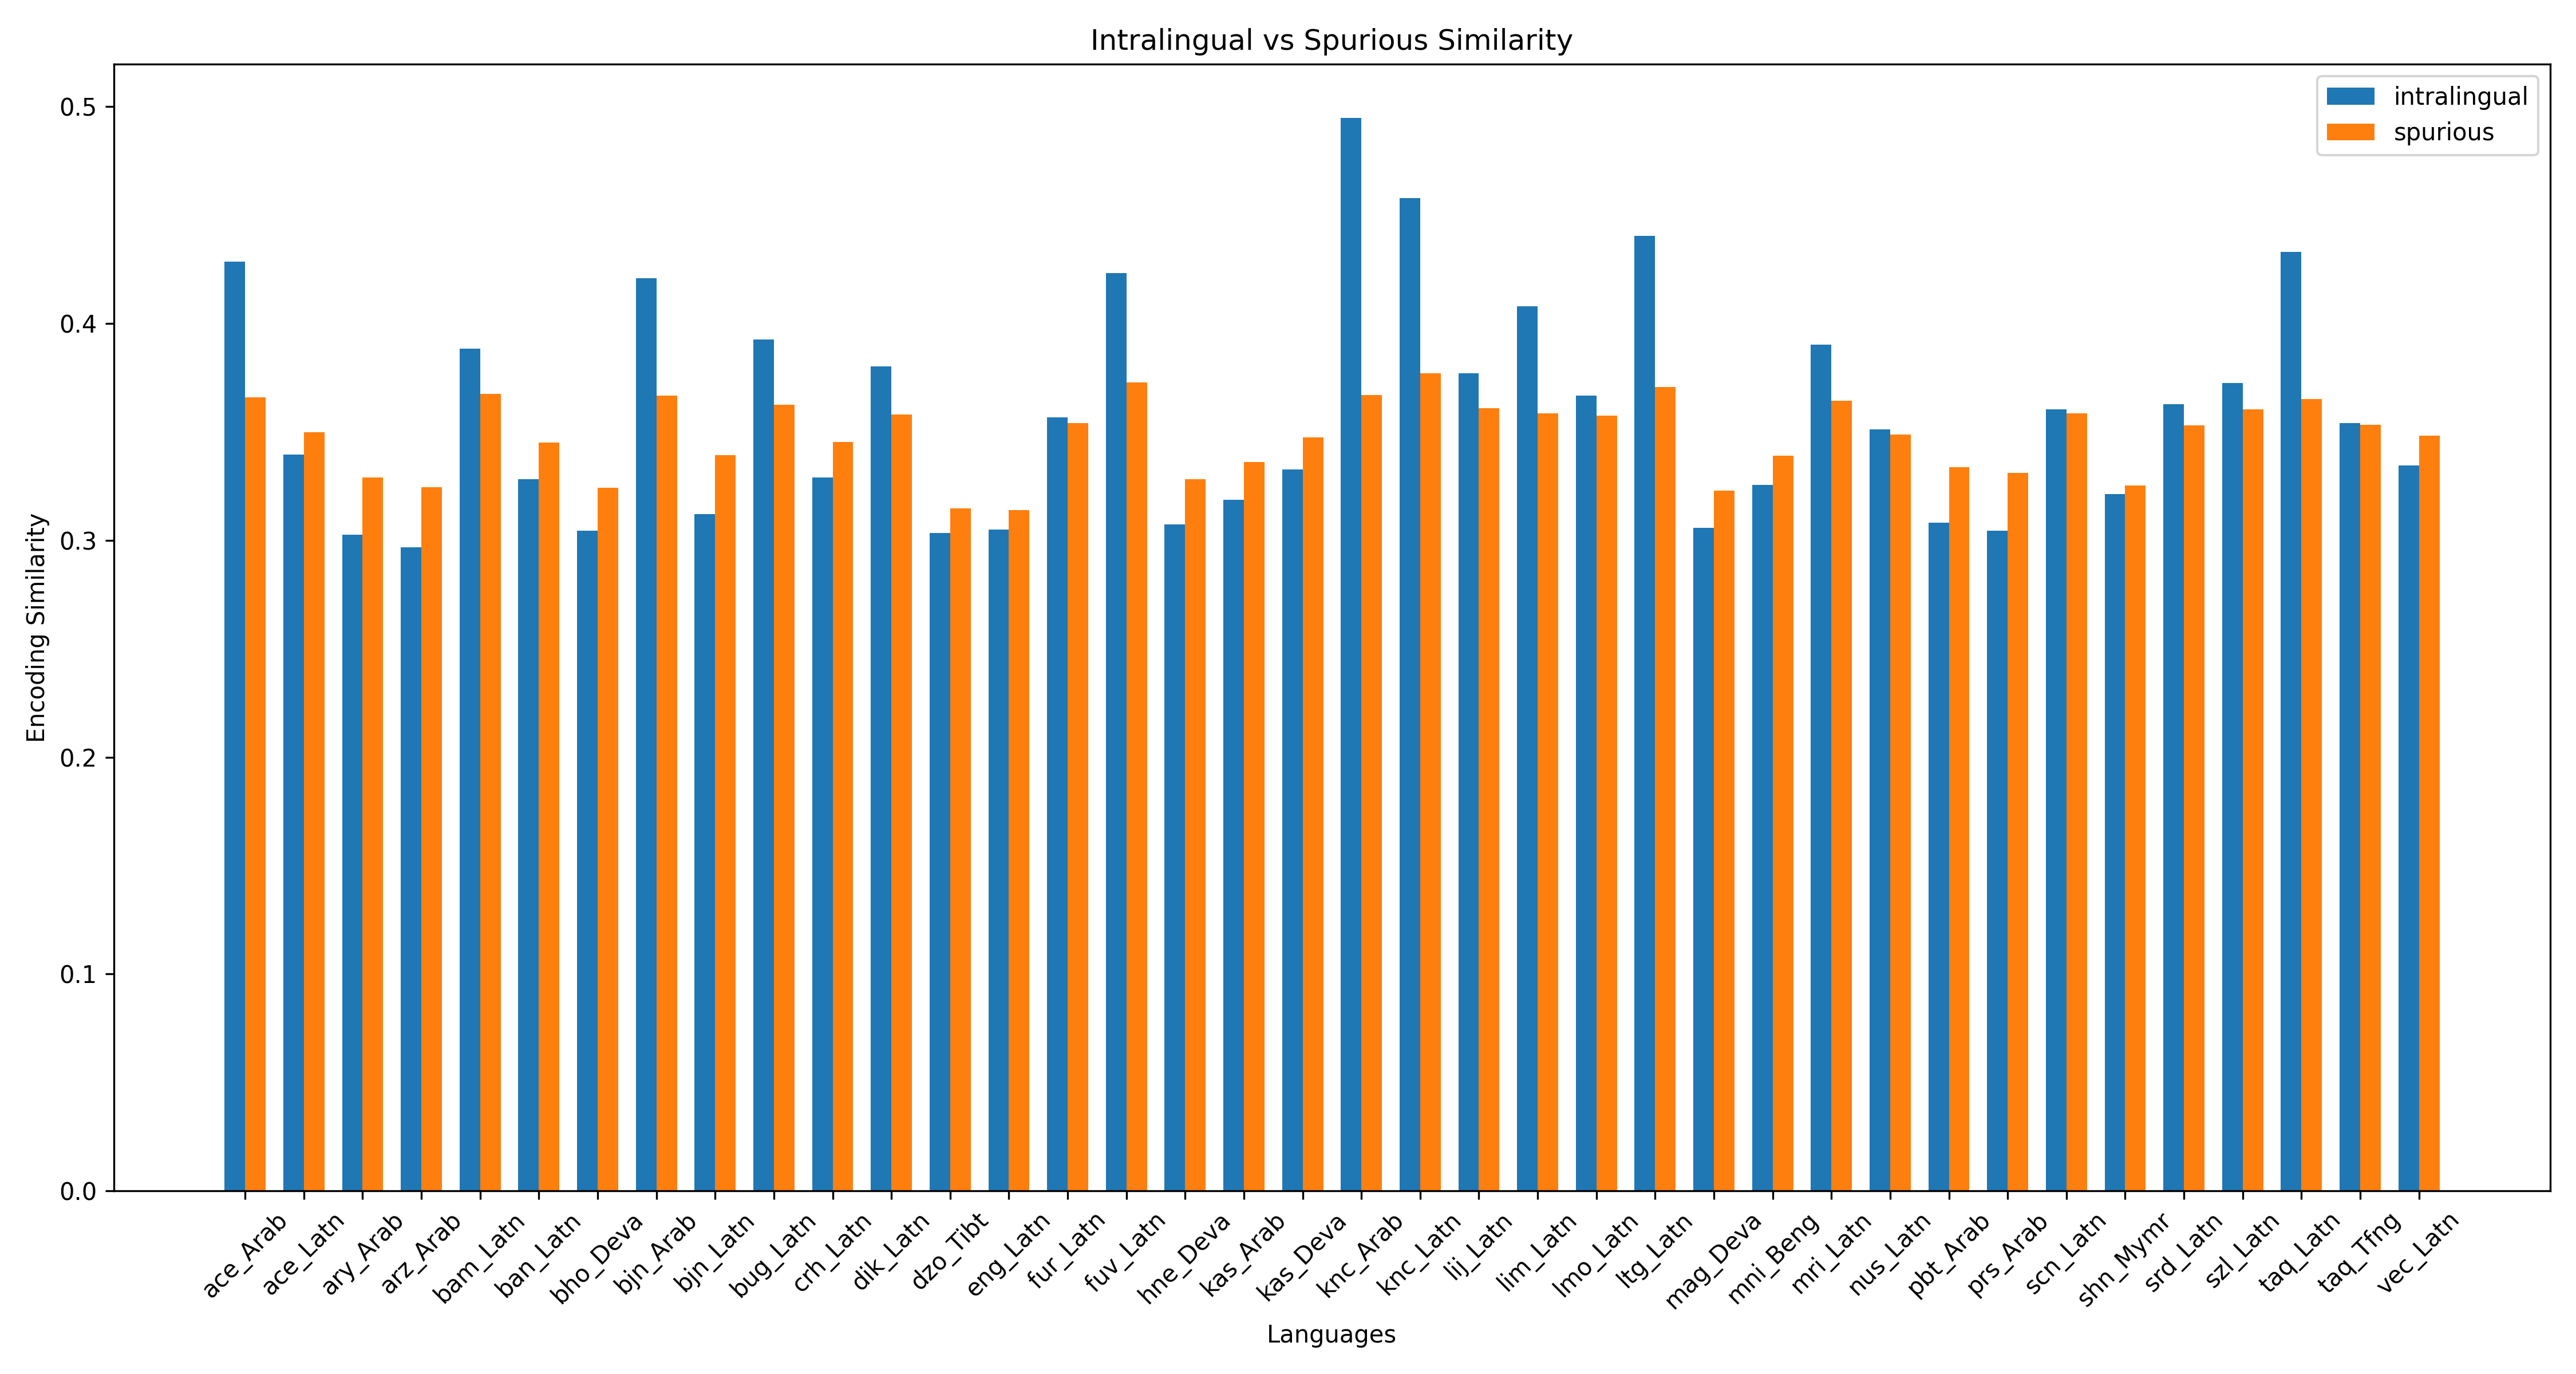
\includegraphics[width=\textwidth]{images/rv3_seed.png}
    
    \caption{Intralingual vs spurious similarity by language in the Seed dataset}
    \label{fig:seed_rv3}
\end{figure}


Somewhat surprisingly, spurious similarity is higher for each of the Europarl languages than intralingual similarity. In other words, randomly matching sentences across languages results shows higher average encoding similarity than randomly matching sentences within each language. Given that each of the Europarl languages is high-resource, it is likely that this behavior is learned during training, and that contrary behavior would lead to higher loss. To put an intuitive gloss on this result, we could speculate that the encoder learns early in training that the language tag of a sentence (e.g. "eng\_Latn") is very important to its job -- encoding an English sentence should be treated as a different task than encoding a Finnish one. After beginning with a naive language-based grouping of sentences, the model eventually shifts its behavior so as to group sentences by their meaning, a strategy which results in the distribution of sentences from the same language across the encoding space. By that point, the similarity of encodings of sentences from the same language is lower on average than the similarity between two random sentences (of similar length). 

The average intralingual similarity in the Europarl dataset is 0.319, while the average spurious similarity is 0.359. [insert same statistical results as above]. In the Seed dataset, the intralingual average is 0.359\footnote{I did double-check these two appearances of 0.359, and it's not a typo, just a numerical coincidence.} and the spurious similarity is 0.348. Intralingual similarity is higher than spurious similarity in the Seed dataset, but not the Europarl one. Again, the resource level of each dataset's languages in NLLB training should be remembered. If we believe the narrative laid out in the previous paragraph, we could place the low-resource Seed languages at an earlier stage of model understanding than the high-resource Europarl languages. The model did not reach a point of mastery with some of the Seed languages to be able to apply its advanced strategy of organizing sentences in space according to their meaning. 

Another feature of the data displayed in the two graphs above is a difference in variance. Both intralingual and spurious similarity seems to vary more greatly across languages in the Seed dataset than in the Europarl dataset. Indeed, the Europarl dataset has a variance of $1.559 * 10^{-4}$ in intralingual similarities, an order of magnitude lower than that of the Seed dataset, $2.542 * 10^{-3}$. The same holds for spurious similarity: in Europarl, $1.220 * 10^{-5}$, and in Seed, $2.911 * 10^{-4}$. What emerges from these observations is a sense that the NLLB model's treatment of Europarl sentences is more stable and consistent than its treatment of Seed sentences. 










